% ─────────────────────────────────────────────────────────────────────────────
% CS3315 Final Project — Conference-paper version (IEEE two-column)
% Aviation Engine Health Monitoring on the NGAFID benchmark
% Iván Barbosa Mejía · NPS MSCS Q3 · 2026
% Numbers sourced from notebooks 01–05 (results/*.csv and figures/).
% Compile: make  (pdflatex → bibtex → pdflatex × 2)
% ─────────────────────────────────────────────────────────────────────────────
\documentclass[conference]{IEEEtran}
\IEEEoverridecommandlockouts

% ── Encoding & fonts ─────────────────────────────────────────────────────────
\usepackage[utf8]{inputenc}
\usepackage[T1]{fontenc}

% ── Math ─────────────────────────────────────────────────────────────────────
\usepackage{amsmath,amssymb}

% ── Figures / tables ─────────────────────────────────────────────────────────
\usepackage{graphicx}
\graphicspath{{../figures/}}   % notebook-generated figures (01–05)
\usepackage{float}
\usepackage{booktabs}
\usepackage{array}
\usepackage{multirow}
\usepackage{tikz}
\usetikzlibrary{arrows.meta, positioning}

% ── Hyperlinks ───────────────────────────────────────────────────────────────
\usepackage{hyperref}
\hypersetup{colorlinks=true, linkcolor=blue, urlcolor=blue, citecolor=blue}
\usepackage{microtype}

% ─────────────────────────────────────────────────────────────────────────────
\title{Classical Machine Learning for Aviation Engine Health Monitoring:\\
       Anomaly Detection and Fault Classification on the NGAFID Benchmark}

\author{
    \IEEEauthorblockN{Iván Barbosa Mejía}
    \IEEEauthorblockA{
        \textit{Department of Computer Science} \\
        \textit{Naval Postgraduate School} \\
        Monterey, California, USA \\
        CS3315 --- Introduction to Machine Learning \& Big Data \\
        \texttt{https://github.com/Barbosa12/NGAFID}
    }
}

\begin{document}
\maketitle

% ─────────────────────────────────────────────────────────────────────────────
\begin{abstract}
General aviation still relies on calendar-based maintenance, which misses faults
that emerge between fixed inspection windows. We study whether \emph{classical}
machine learning on flight-level statistical features can support condition-based
maintenance, using the National General Aviation Flight Information Database
(NGAFID), a real-world benchmark of $11{,}446$ Cessna-172 flights labeled with 19
fault categories. We cast the problem as a two-stage pipeline: binary Anomaly
Detection (AD) followed by 19-class Fault Classification (FC). Five classical
models are trained over a hierarchy of representations---global per-sensor
statistics, temporal segments, and physics-based inter-cylinder features---and
compared with deep learning (DL) figures reported in the literature. Our best
classical system reaches $F1=0.703$ on AD (tuned ensemble, 224 features), within
$1.8$ points of a published temporal DL model, but FC tops out at $F1=0.207$ for
a flat classifier and $F1=0.459$ for an Oracle hierarchical ceiling. We trace this
asymmetry to \emph{target-component sparsity}: fault-discriminative information
lives in low-variance principal components (PC9, PC19--23) that global statistics
discard. An end-to-end error decomposition shows that fault \emph{typing}, not
detection, is the bottleneck (the largest single error mode). We report the DL
comparison transparently: its source preprint was later withdrawn by its authors
over metric-computation flaws, so those numbers are treated as indicative only.
All results derive from the project notebooks~01--05.
\end{abstract}

\begin{IEEEkeywords}
anomaly detection, fault classification, time series, aviation maintenance,
NGAFID, imbalanced learning.
\end{IEEEkeywords}

% ─────────────────────────────────────────────────────────────────────────────
\section{Introduction}
\label{sec:intro}
Modern aircraft continuously log dozens of sensor channels through their engine
control units, yet general aviation maintenance remains \emph{calendar-based}:
inspections occur at fixed intervals regardless of component condition. This
reactive paradigm misses faults that emerge between windows, creating safety
risks and costly unscheduled groundings. Machine learning offers a path toward
\emph{condition-based} maintenance, flagging anomalous flights and identifying
likely fault types directly from telemetry.

We use the NGAFID benchmark~\cite{ngafid2021}, a real (non-simulated) dataset
from an active Cessna-172 flight school, and address two research questions:
\textbf{(RQ1)} can a classical classifier trained on statistics extracted from
the full flight profile reliably separate healthy from anomalous flights? and
\textbf{(RQ2)} given an anomalous flight, can the same approach identify which of
19 fault types is responsible? We hypothesize that \emph{global} statistics
suffice for AD (whole-flight health state), but fail on FC because fault
signatures are \emph{local} micro-patterns that global aggregation discards. Both
tasks are composed into an end-to-end (E2E) 20-class pipeline.

Our contributions are: (i) a systematic evaluation of five classical models over
a hierarchy of feature representations on NGAFID; (ii) empirical evidence for
\emph{target-component sparsity} as the structural reason FC is hard; (iii) an
Oracle hierarchical experiment that raises the classical FC ceiling from $0.116$
to $0.459$; and (iv) an E2E error decomposition that locates fault classification
as the dominant bottleneck. Every figure and table in this paper is reproduced
from the project notebooks 01 (EDA), 02 (dataset/feature build), 03 (AD), 04 (FC),
and 05 (E2E).

% ─────────────────────────────────────────────────────────────────────────────
\section{Dataset and Feature Engineering}
\label{sec:data}

\subsection{NGAFID Benchmark}
NGAFID correlates 23-channel, 1\,Hz telemetry with verified unscheduled
maintenance records~\cite{ngafid2021}. We use the 2-day benchmark subset:
$11{,}446$ flights, nearly balanced at the binary level---$5{,}844$ healthy
($51.1\%$) and $5{,}602$ anomalous ($48.9\%$)---but \emph{severely long-tailed}
at the fault level, where the two largest categories (rocker-cover and intake-
gasket damage) dominate and the smallest classes have barely a hundred flights,
an imbalance ratio of roughly $38{:}1$ (Fig.~\ref{fig:classdist}). Each flight is
interpolated to a fixed $\mathbf{X}\in\mathbb{R}^{2048\times 23}$ matrix via cubic
spline. The 23 channels span electrical (\texttt{volt}, \texttt{amp}), fuel,
engine (\texttt{FFlow}, \texttt{OilT}, \texttt{OilP}, \texttt{RPM}), four-cylinder
CHT and EGT, flight state, and ambient temperature. All experiments use 5-fold
stratified cross-validation with strict per-aircraft isolation to prevent
leakage; standardization is fit on the training split only.

\begin{figure*}[t]
    \centering
    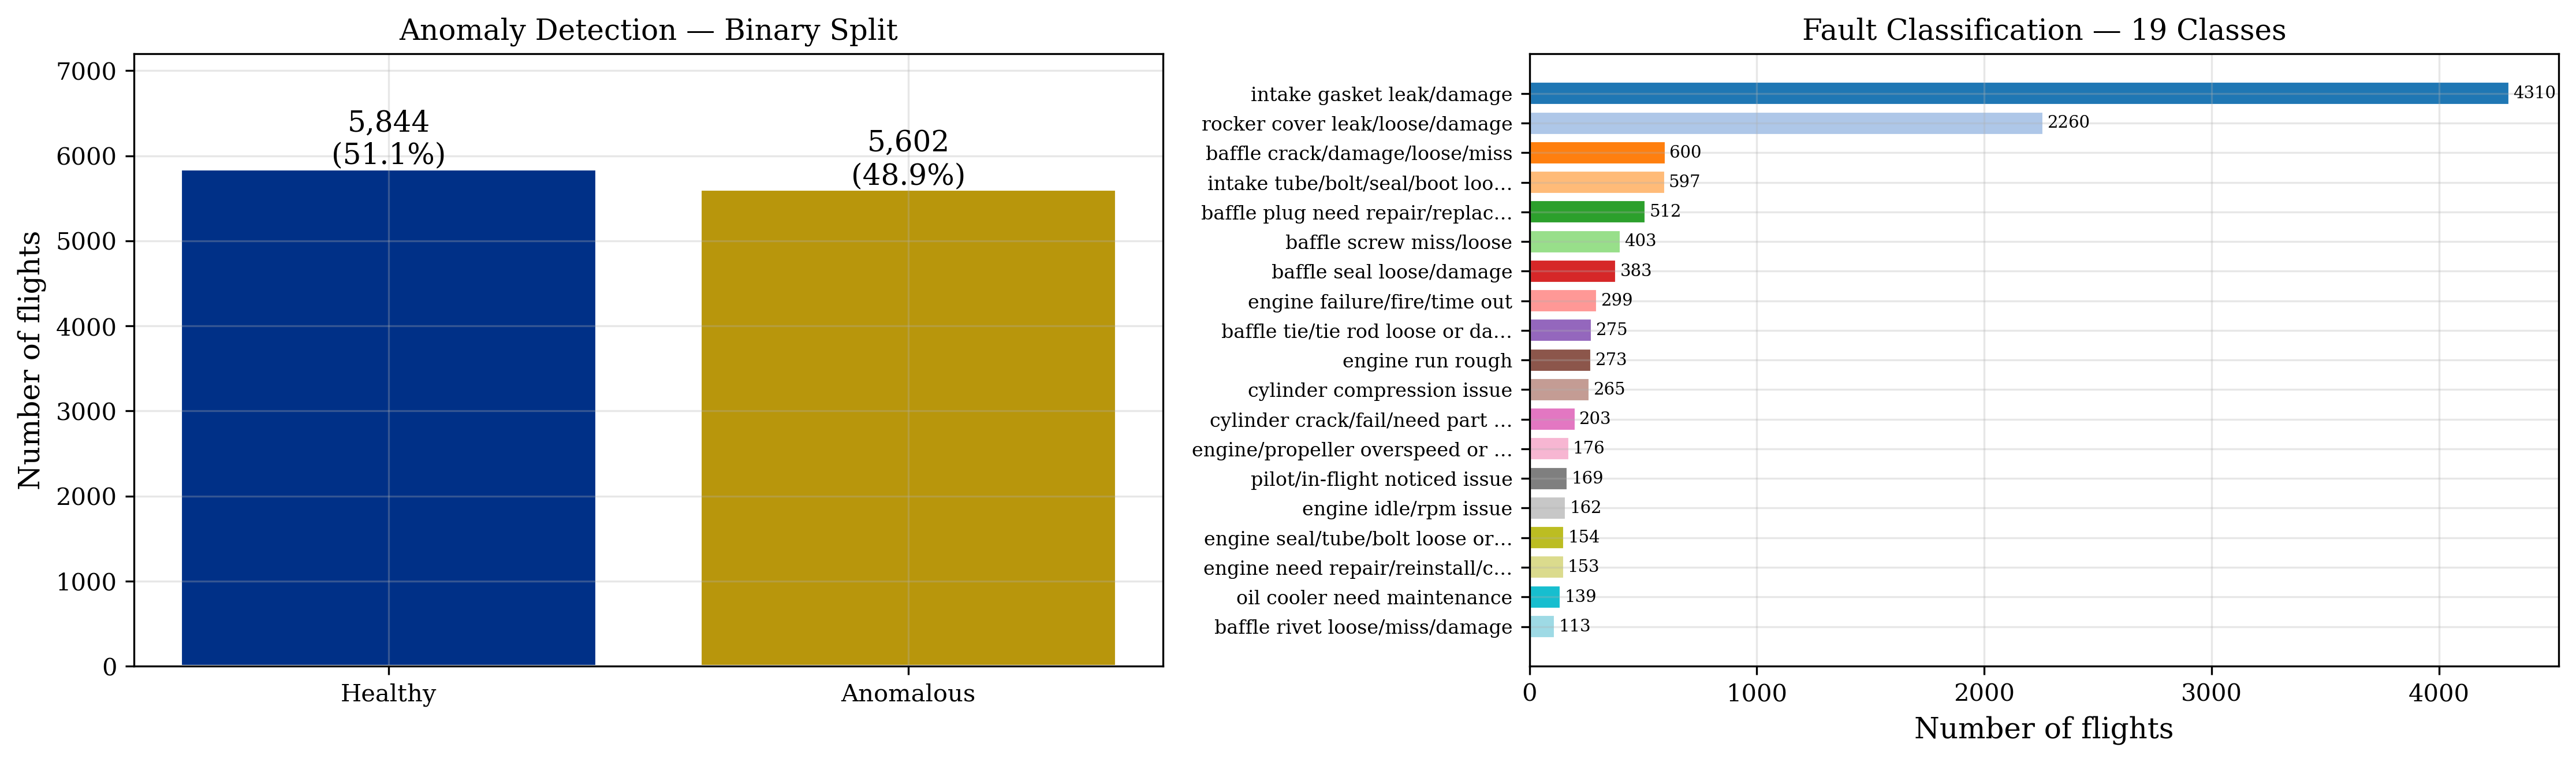
\includegraphics[width=0.92\textwidth]{class-distribution.png}
    \caption{NGAFID benchmark subset (notebook~01). Left: the binary AD split is
             nearly balanced. Right: the 19 fault classes are severely
             long-tailed, with the two head classes dominating---the core
             difficulty for fault classification.}
    \label{fig:classdist}
\end{figure*}

\subsection{Feature Representations}
We compress each variable-length flight into a fixed feature vector
(Table~\ref{tab:repr}). Representation~B computes eight statistics
($\mu,\sigma,\min,\max,\text{range},\text{skew},\text{kurt},\hat\beta$) per
channel, giving $23\times 8 = 184$ features. Representation~$F_{++}$ adds
\emph{cross-physical} inter-cylinder features (CHT/EGT spread, coefficient of
variation, pairwise ratios), reaching 224 features; XGBoost gain-based selection
then reduces this to 60 (Repr.~F). Segmented variants ($B_{\text{seg}}$) apply
Repr.~B to $N$ equal flight segments to inject coarse temporal ordering, and
temporal-shape transforms (MiniRocket~G~\cite{minirocket2021}, tsfresh~H
\cite{tsfresh2018}) were also explored.

\begin{table}[t]
    \centering
    \caption{Feature representations explored (notebook~02).}
    \label{tab:repr}
    \footnotesize
    \begin{tabular}{llc}
        \toprule
        \textbf{Repr.} & \textbf{What it captures} & \textbf{Dim.} \\
        \midrule
        B               & Global per-sensor statistics          & 184 \\
        $B_{\text{seg}}$ & Repr.~B over $N$ flight segments      & 552--1840 \\
        $F_{++}$        & B $+$ cross-cylinder asymmetry/ratios  & 224 \\
        F               & $F_{++}$ $+$ XGB gain selection        & 60 \\
        G               & MiniRocket random kernels             & $\sim$10k \\
        H               & tsfresh (ACF, FFT, entropy)           & var \\
        \bottomrule
    \end{tabular}
\end{table}

\subsection{Why Fault Classification is Hard}
\label{subsec:sparsity}
Projecting Repr.~B into principal-component space exposes the structural obstacle
(Fig.~\ref{fig:sparsity}). The high-variance components PC1--PC2 capture
operational variability common to healthy and anomalous flights (altitude,
throttle, ambient temperature) and are nearly \emph{non-discriminative}. The
components that actually separate healthy from anomalous---PC9 and PC19--PC23 by
$F$-statistic---each contribute very little to total variance. Fault-relevant
information is thus \emph{sparse} and buried beneath operational variance, so any
global statistic that emphasizes high-variance directions discards exactly the
signal FC needs. This is the empirical basis for our hypothesis.

\begin{figure*}[t]
    \centering
    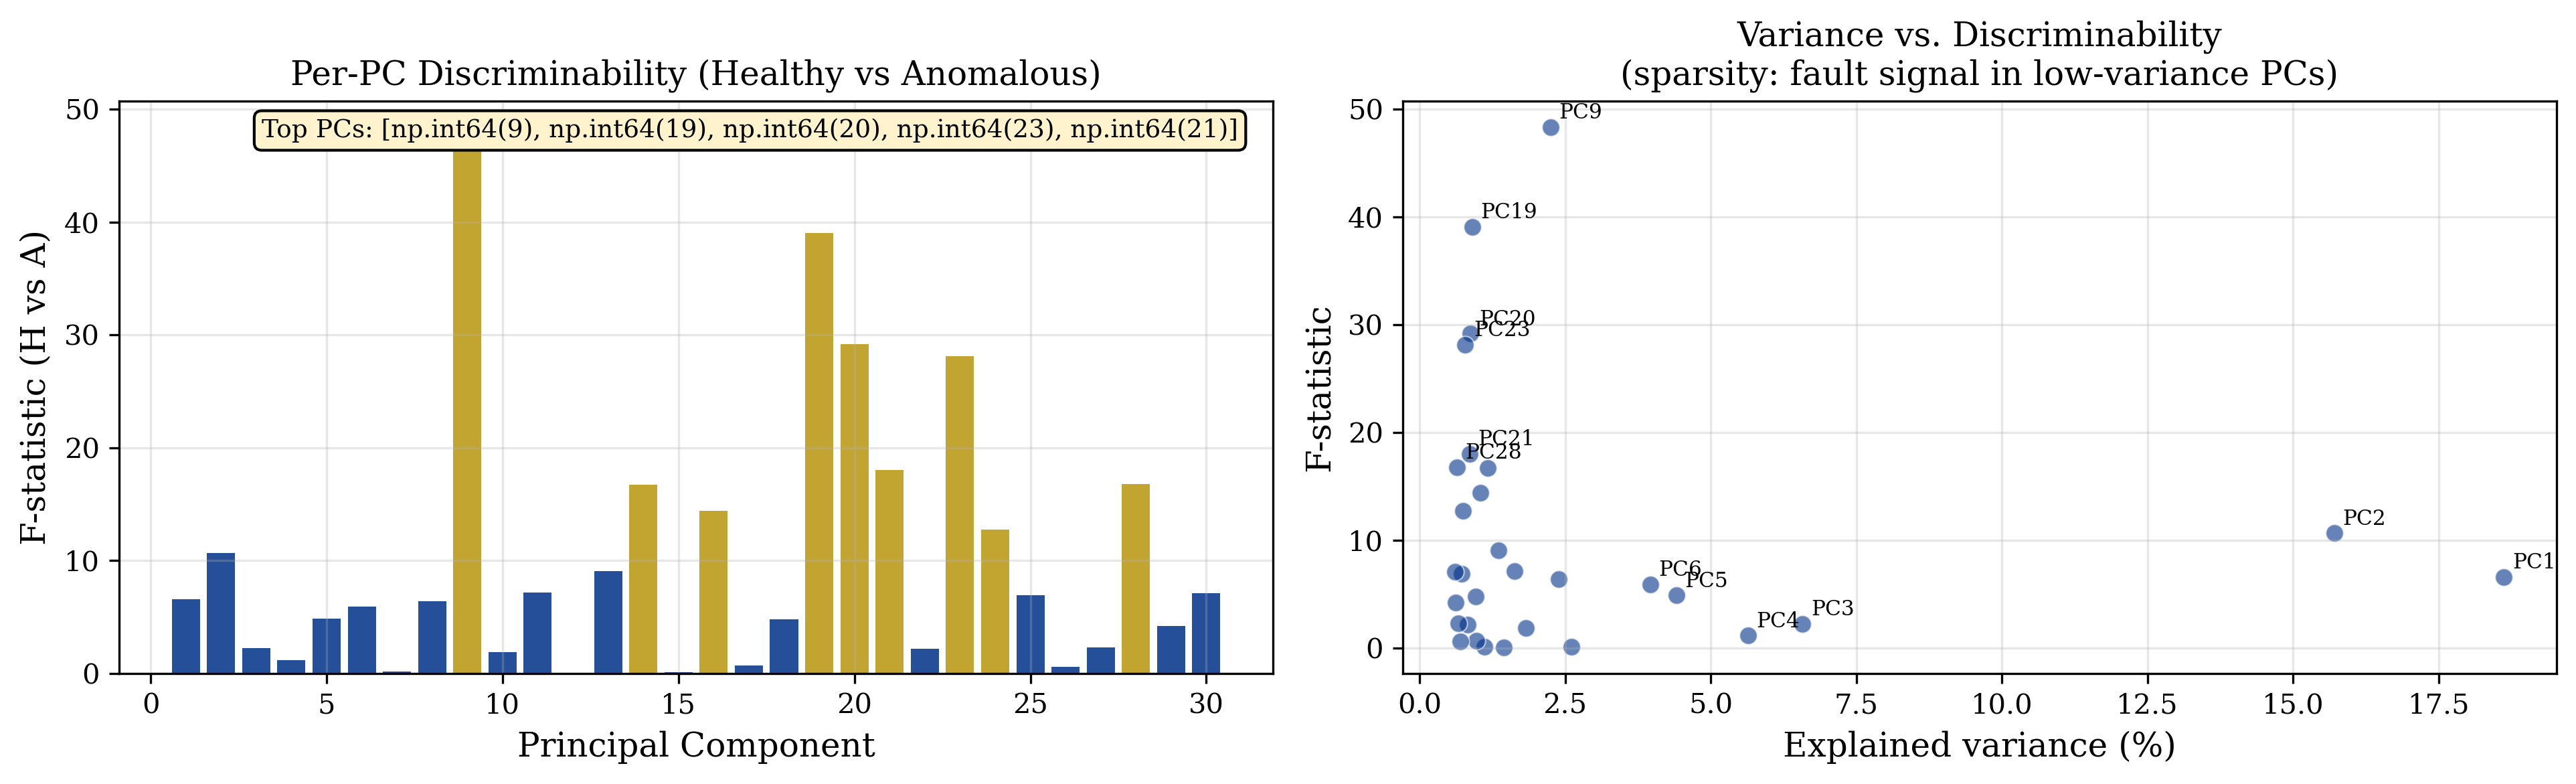
\includegraphics[width=0.92\textwidth]{target-component-sparsity.png}
    \caption{Target-component sparsity (notebook~01). Left: per-PC
             discriminability ($F$-statistic, healthy vs.\ anomalous)---the most
             discriminative components are high-index. Right: discriminability
             vs.\ explained variance---the high-variance PC1--PC2 are weakly
             discriminative, while the discriminative PCs carry little variance.}
    \label{fig:sparsity}
\end{figure*}

% ─────────────────────────────────────────────────────────────────────────────
\section{Methodology}
\label{sec:method}
The 20-class problem ($0=$healthy, $1\text{--}19=$faults) is decomposed into a
two-stage cascade (Fig.~\ref{fig:pipeline}). Stage~1 (AD) is binary; only flights
flagged anomalous proceed to Stage~2 (FC). The decomposition reflects the opposing
inductive biases of the two tasks: AD benefits from global whole-flight context,
while FC requires local fault resolution~\cite{lmsd2025}.

\begin{figure}[t]
    \centering
    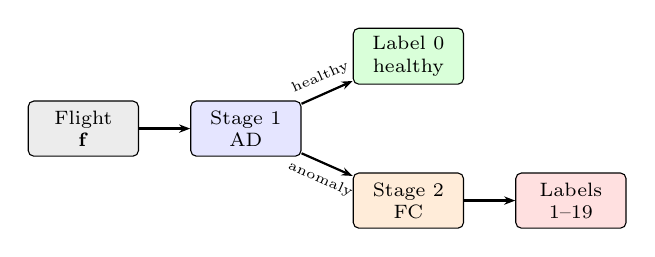
\begin{tikzpicture}[
        every node/.style={align=center, font=\scriptsize},
        box/.style={draw, rounded corners=2pt, minimum width=1.4cm,
                    minimum height=0.7cm, inner sep=3pt},
        arr/.style={-{Stealth[length=4pt]}, thick},
        node distance=0.4cm and 0.65cm
    ]
        \node[box, fill=gray!15]  (raw) {Flight\\$\mathbf{f}$};
        \node[box, fill=blue!10, right=of raw] (ad) {Stage 1\\AD};
        \node[box, fill=green!15, above right=0.2cm and 0.65cm of ad] (h) {Label 0\\healthy};
        \node[box, fill=orange!15, below right=0.2cm and 0.65cm of ad] (fc) {Stage 2\\FC};
        \node[box, fill=red!12, right=of fc] (fault) {Labels\\1--19};
        \draw[arr] (raw) -- (ad);
        \draw[arr] (ad) -- node[above,font=\tiny,sloped]{healthy} (h);
        \draw[arr] (ad) -- node[below,font=\tiny,sloped]{anomaly} (fc);
        \draw[arr] (fc) -- (fault);
    \end{tikzpicture}
    \caption{Two-stage diagnosis pipeline (notebook~05).}
    \label{fig:pipeline}
\end{figure}

\textbf{Models.} We evaluate Logistic Regression (LR), Linear SVM, XGBoost
(XGB)~\cite{xgboost2016}, Random Forest (RF), and KNN, all in
scikit-learn~\cite{sklearn2011}, with class weighting for imbalance; a soft-voting
\emph{Ensemble} (LR$+$XGB) is also tuned. \textbf{Oracle hierarchy.} Ward
clustering groups the 19 classes into $K{=}4$ physically coherent super-groups; a
per-group XGB is trained, using ground-truth group membership at test time to
obtain an upper bound. \textbf{Metrics.} The primary metric is macro-$F1$; for AD
we also report AUC and the False Negative Rate (FNR), the safety-critical miss
rate. \textbf{DL reference.} We compare against ConvTokMHSA, MMK~Net, and the LMSD
framework as reported in the literature.\footnote{The deep learning figures are
reproduced from the LMSD preprint~\cite{lmsd2025}, which was subsequently
\emph{withdrawn} by its authors, who stated that ``significant methodological
flaws have been identified in the experimental validation and metric-computation
procedures.'' We present these numbers as indicative reference points, not
validated upper bounds, and interpret all gaps accordingly.}

% ─────────────────────────────────────────────────────────────────────────────
\section{Results}
\label{sec:results}

\subsection{Anomaly Detection}
Table~\ref{tab:ad} reports 5-fold AD performance. On Repr.~B the tuned Ensemble
leads at $F1=0.691$; adding cross-cylinder features ($F_{++}$) raises the best
classical result to $F1=0.703$ with $\text{AUC}=0.767$ and $\text{FNR}=0.307$
(Fig.~\ref{fig:adroc}). This is \emph{competitive} with temporal DL: it trails the
best reported model (ConvTokMHSA, $0.799$) by $9.6$ points but is within $1.8$
points of MMK~Net ($0.721$). Feature importance (Fig.~\ref{fig:adfeat}) is
dominated by oil-pressure statistics (\texttt{E1 OilP\_std}, \texttt{\_range},
\texttt{\_mean}), matching the physical role of oil pressure as the primary
engine-health indicator, followed by electrical and cross-cylinder features.

\begin{table}[t]
    \centering
    \caption{Anomaly Detection (5-fold CV). Best classical per metric in
             \textbf{bold}; DL figures are indicative (footnote~1).}
    \label{tab:ad}
    \footnotesize
    \begin{tabular}{llcccc}
        \toprule
        \textbf{Model} & \textbf{Repr.} & \textbf{F1} & \textbf{AUC} & \textbf{FNR} & \textbf{FPR} \\
        \midrule
        \multicolumn{6}{l}{\textit{Classical (this work, Repr.~B)}} \\
        Ensemble      & B       & 0.691 & 0.754 & 0.322 & 0.296 \\
        Logistic Reg. & B       & 0.679 & 0.730 & 0.308 & 0.333 \\
        XGBoost       & B       & 0.675 & 0.742 & 0.330 & 0.321 \\
        Linear SVM    & B       & 0.675 & 0.726 & 0.347 & 0.303 \\
        Random Forest & B       & 0.651 & 0.707 & 0.400 & 0.298 \\
        KNN           & B       & 0.545 & 0.562 & 0.477 & 0.431 \\
        \midrule
        \textbf{Ensemble (best)} & $F_{++}$ & \textbf{0.703} & \textbf{0.767} & \textbf{0.307} & \textbf{0.287} \\
        \midrule
        \multicolumn{6}{l}{\textit{DL benchmarks (indicative)~\cite{lmsd2025}}} \\
        ConvTokMHSA   & raw & 0.799 & --- & 0.163 & --- \\
        InceptionTime~\cite{inceptiontime2020} & raw & 0.784 & --- & 0.196 & --- \\
        MMK Net       & raw & 0.721 & --- & 0.298 & --- \\
        \bottomrule
    \end{tabular}
\end{table}

\begin{figure}[t]
    \centering
    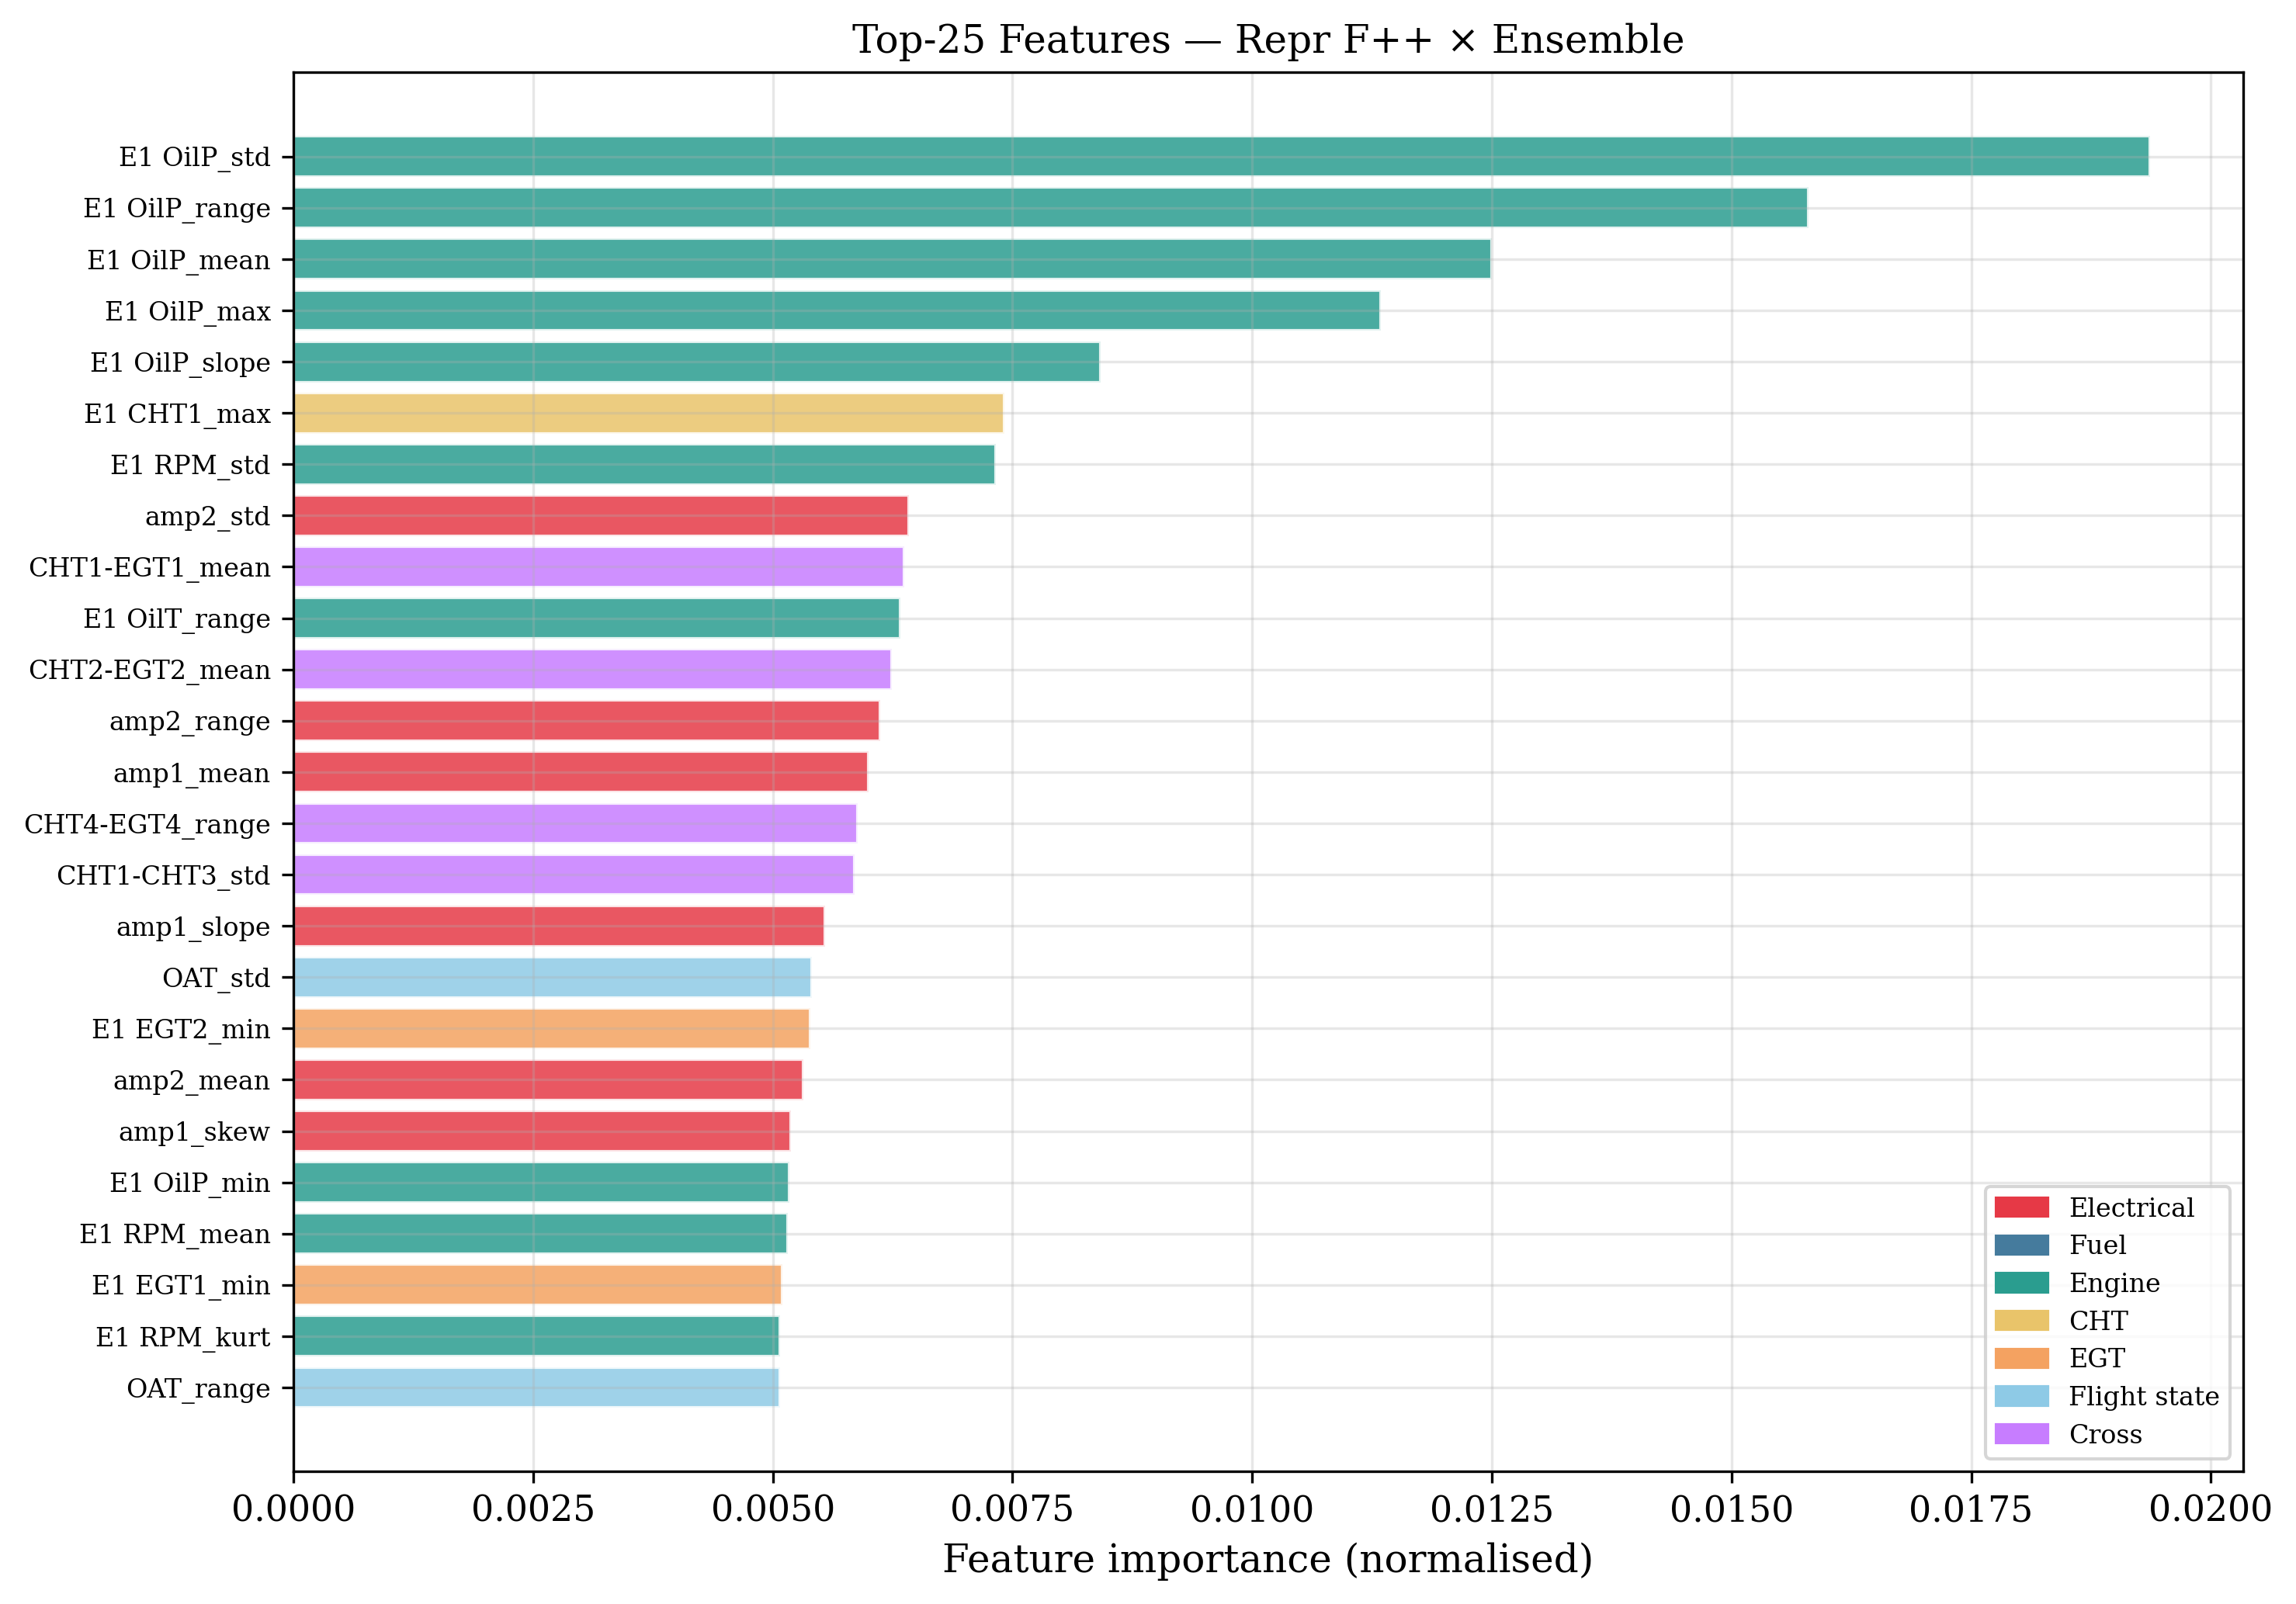
\includegraphics[width=0.83\columnwidth]{ad-feature-importance.png}
    \caption{AD feature importance, tuned Ensemble on $F_{++}$ (notebook~03).
             Oil-pressure statistics dominate; colors denote sensor groups.}
    \label{fig:adfeat}
\end{figure}

\begin{figure*}[t]
    \centering
    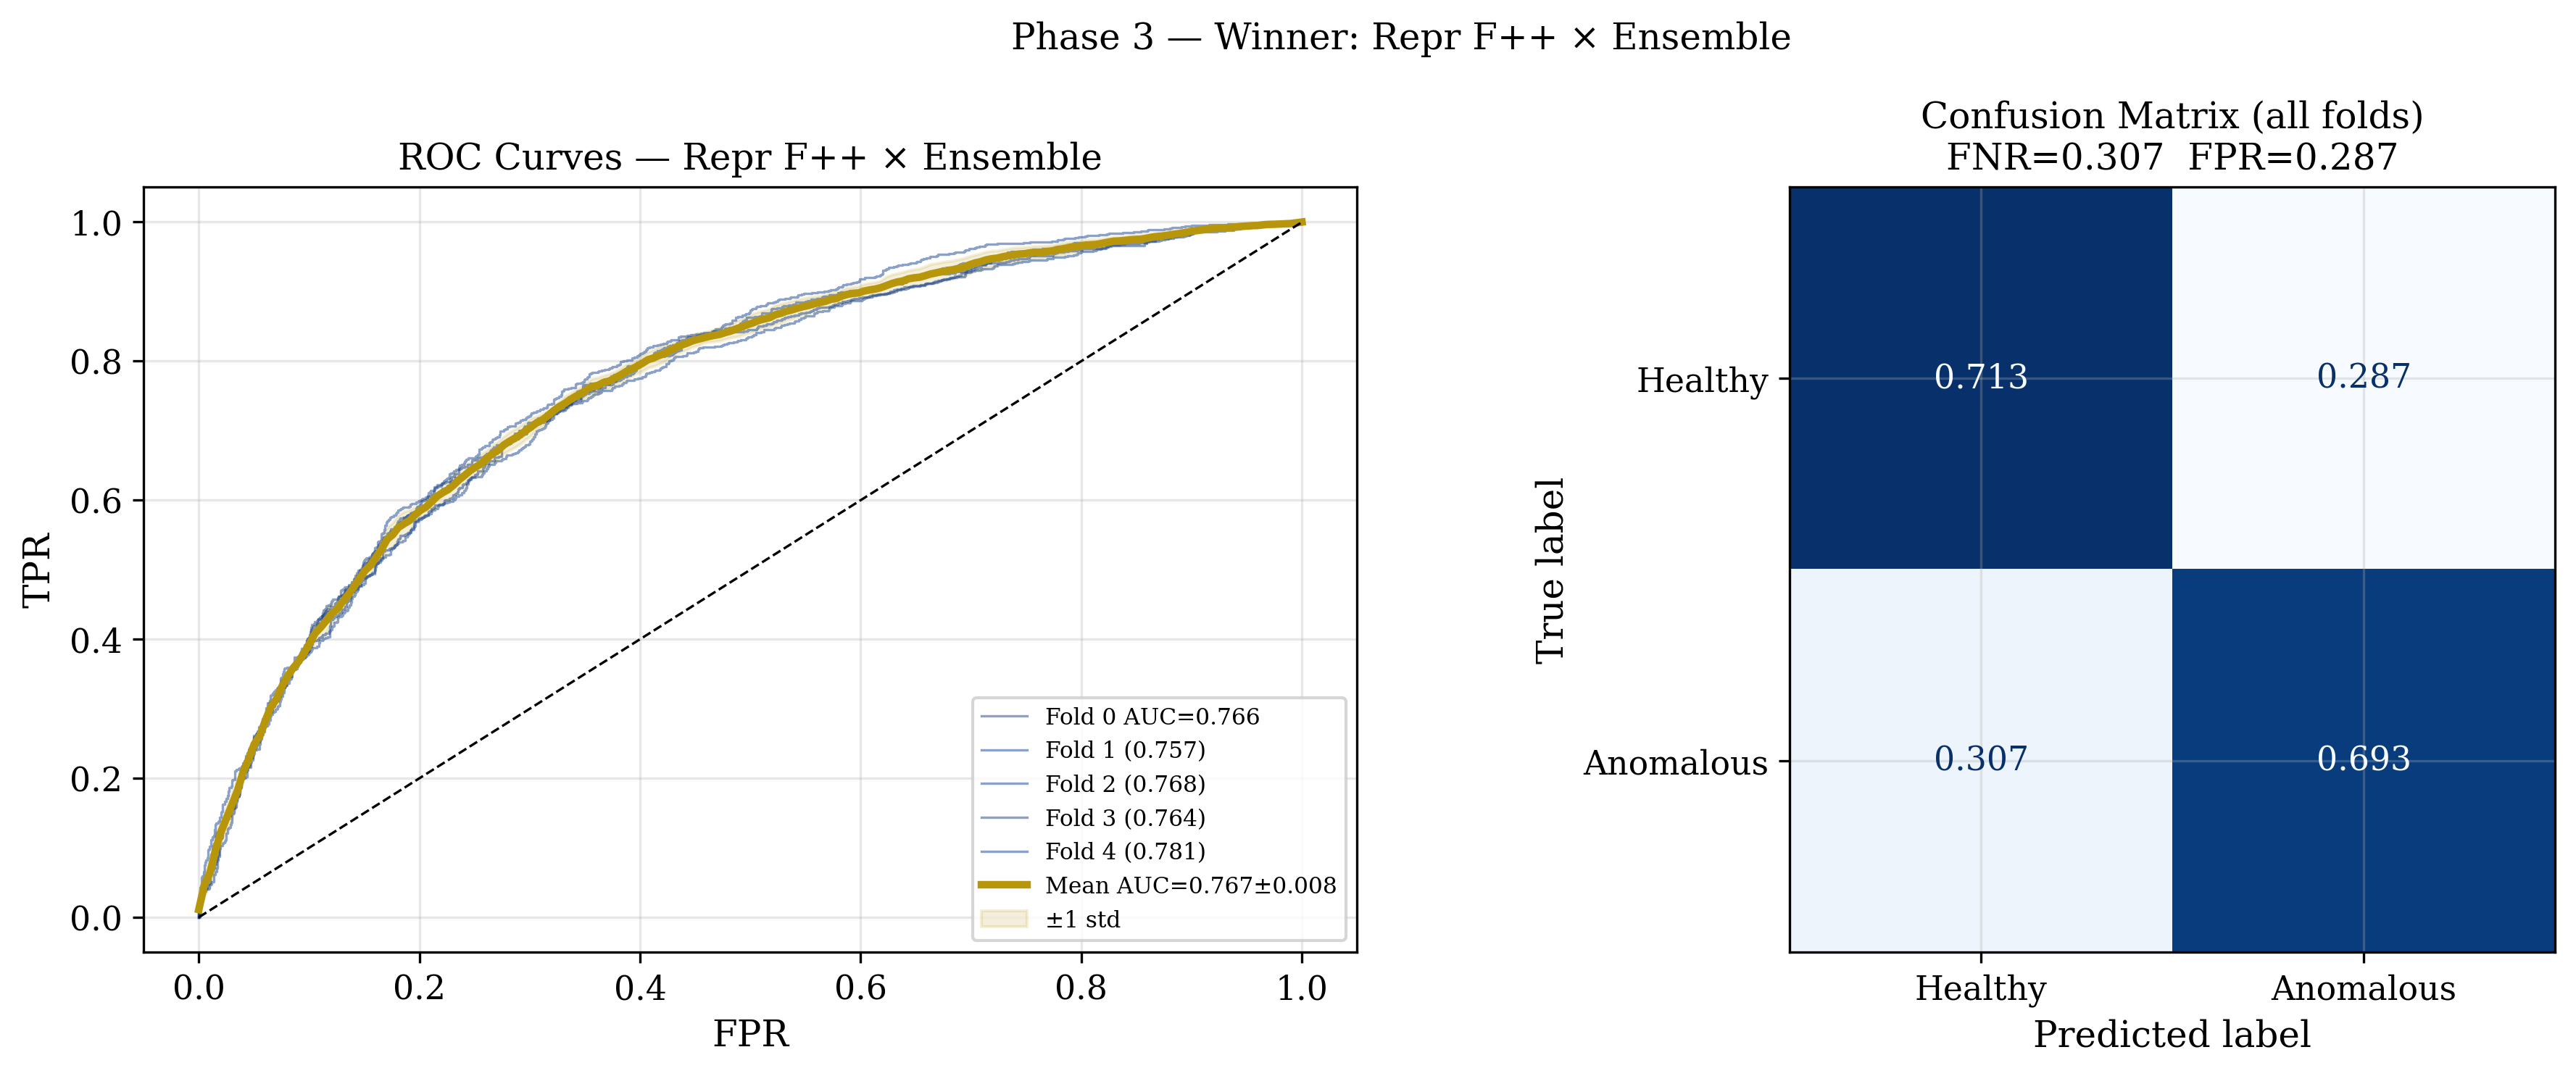
\includegraphics[width=0.86\textwidth]{ad-phase3-roc-cm.png}
    \caption{AD winner---Ensemble on $F_{++}$ (notebook~03). Left: per-fold ROC
             (mean $\text{AUC}=0.767\pm0.008$). Right: confusion matrix
             ($\text{FNR}=0.307$, $\text{FPR}=0.287$); $69.3\%$ of anomalous
             flights are caught.}
    \label{fig:adroc}
\end{figure*}

\subsection{Fault Classification}
FC is markedly harder (Table~\ref{tab:fc}). On the anomalous flights, flat XGBoost
on Repr.~B reaches only $F1=0.116$ (default) and $0.176$ (tuned); the best flat
classical result, XGBoost on $F_{++}$, attains $F1=0.207$. Per-class analysis
(Fig.~\ref{fig:fcperclass}) shows the long-tail effect directly: only the two head
classes clear $F1>0.30$, most classes land in a $0.10$--$0.30$ ``partial'' band,
and per-class $F1$ correlates with training-set size---a textbook imbalance
signature. Hierarchical grouping helps: an Oracle $K{=}4$ partition lifts the
ceiling to $F1=0.459$ (Fig.~\ref{fig:fcladder}), but the realistic cascade variant
($0.172$) confirms that the gain depends on knowing the coarse fault group. Even
the Oracle ceiling trails the best reported DL model (MMK~Net, $0.623$) by $16$
points; tellingly, global-attention ConvTokMHSA ($0.208$) barely matches our flat
XGBoost, confirming that whole-flight context does not help fault typing.

\begin{table}[t]
    \centering
    \caption{Fault Classification (5-fold CV, macro-$F1$, notebook~04).}
    \label{tab:fc}
    \footnotesize
    \begin{tabular}{llc}
        \toprule
        \textbf{Model} & \textbf{Repr.} & \textbf{F1 macro} \\
        \midrule
        XGBoost (default)        & B       & 0.116 \\
        XGBoost (tuned)          & B       & 0.176 \\
        \textbf{XGBoost (tuned, best flat)} & $F_{++}$ & \textbf{0.207} \\
        XGB cascade $K{=}4$      & $F_{++}$ & 0.172 \\
        \textbf{Oracle $K{=}4$ (ceiling)}   & $F_{++}$ & \textbf{0.459} \\
        \midrule
        MMK Net (indicative)~\cite{lmsd2025}   & raw & 0.623 \\
        ConvTokMHSA (indicative)               & raw & 0.208 \\
        \bottomrule
    \end{tabular}
\end{table}

\begin{figure*}[t]
    \centering
    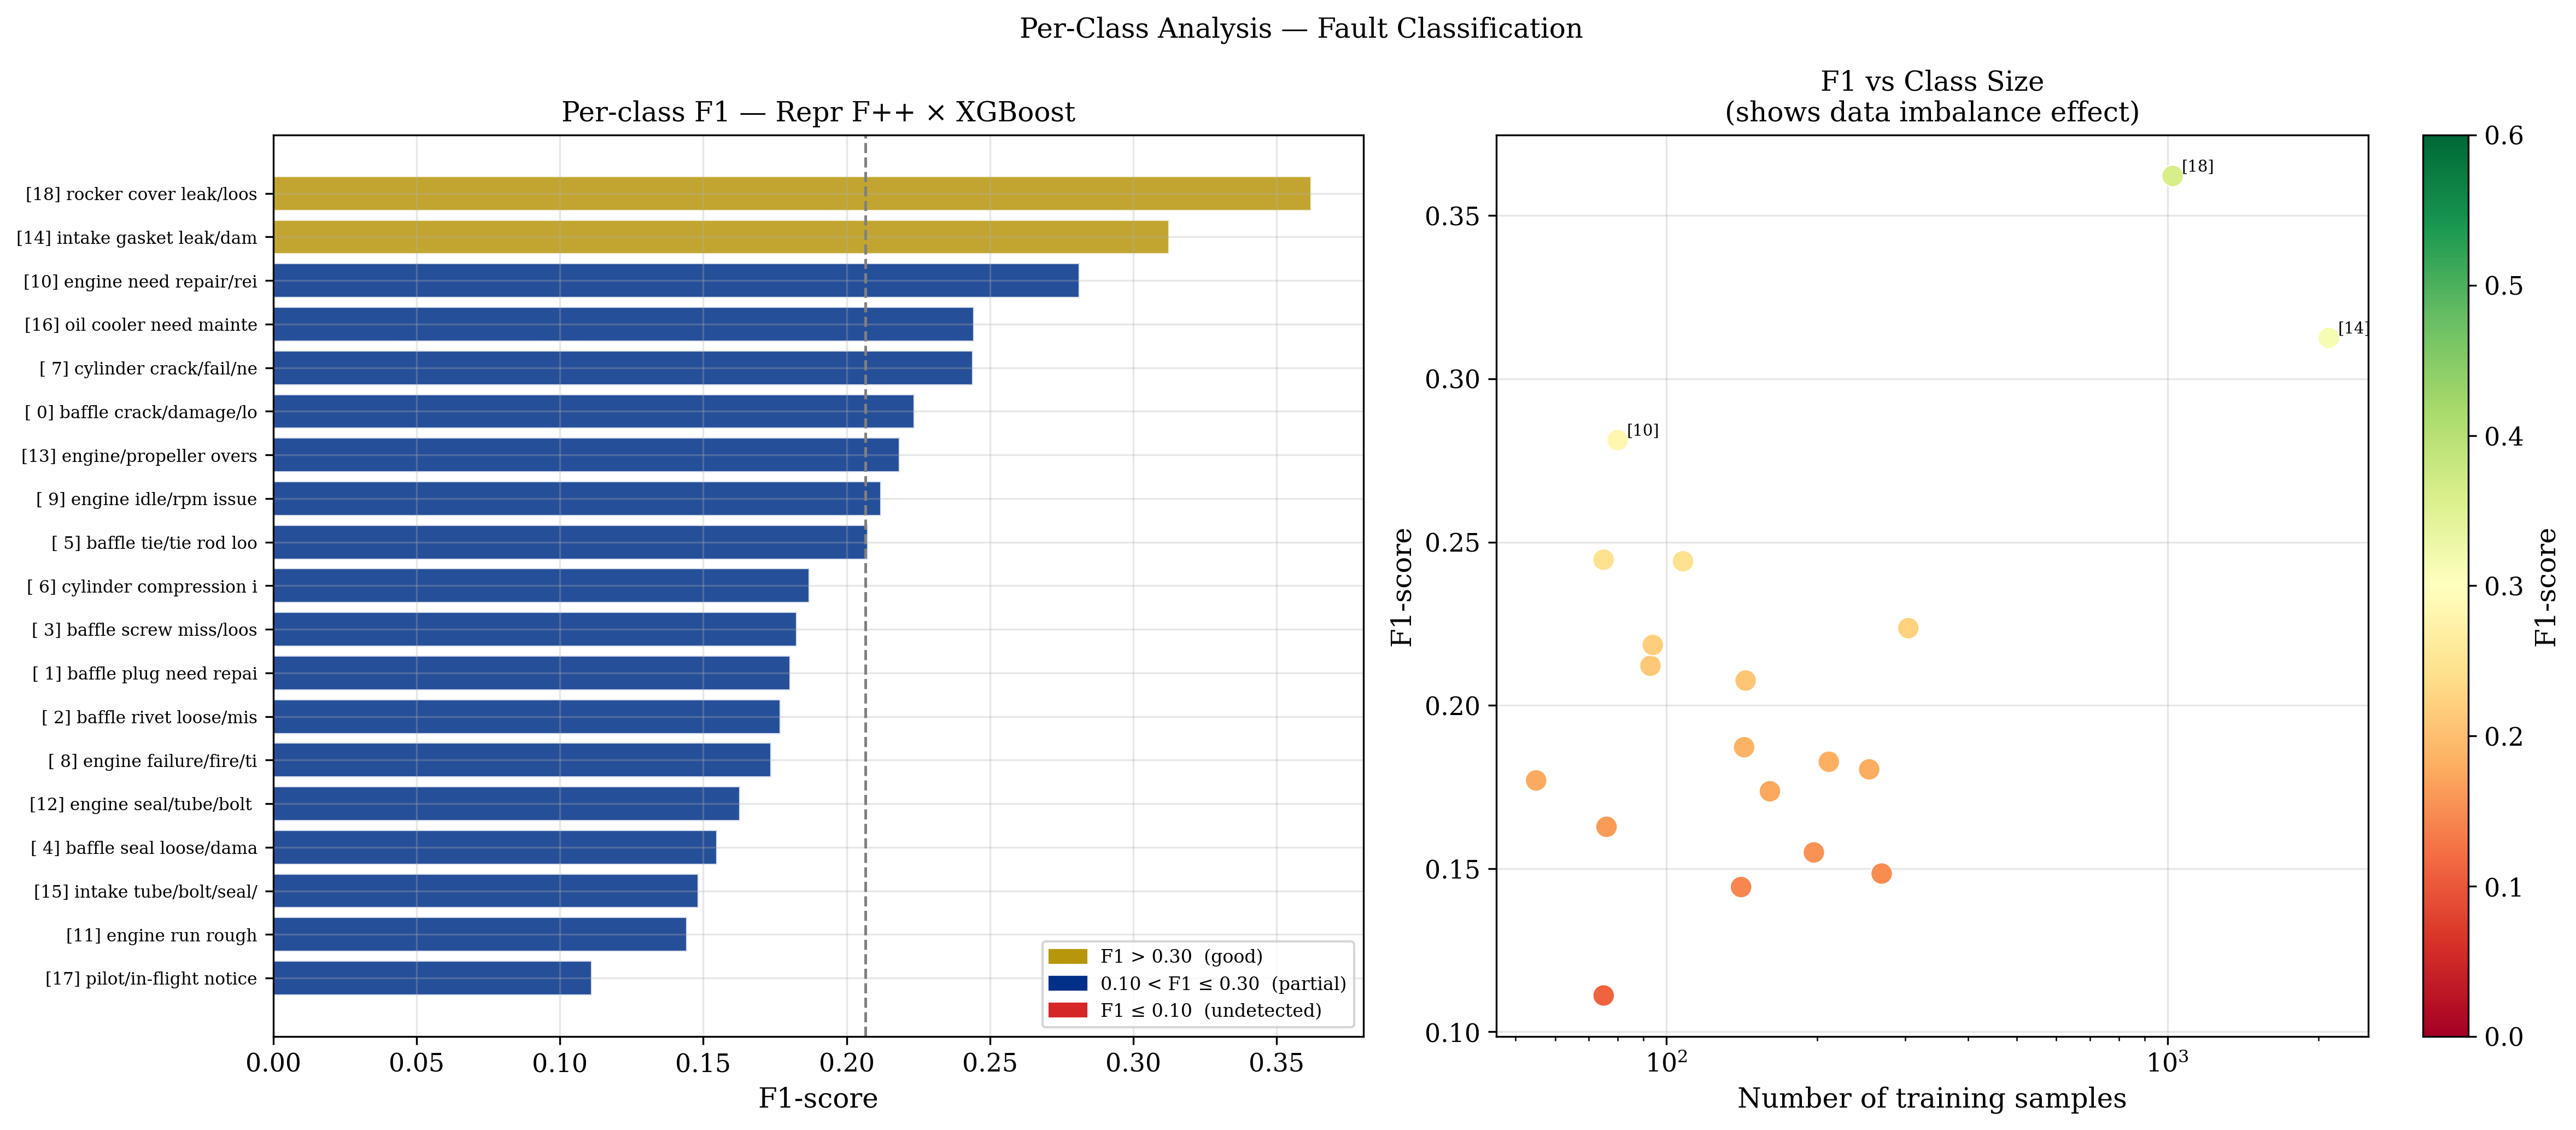
\includegraphics[width=0.88\textwidth]{fc-per-class-f1.png}
    \caption{Per-class FC, best flat model XGBoost on $F_{++}$ (notebook~04).
             Left: per-class $F1$; only head classes exceed $0.30$. Right: $F1$
             vs.\ training-set size, exposing the imbalance effect.}
    \label{fig:fcperclass}
\end{figure*}

\begin{figure}[t]
    \centering
    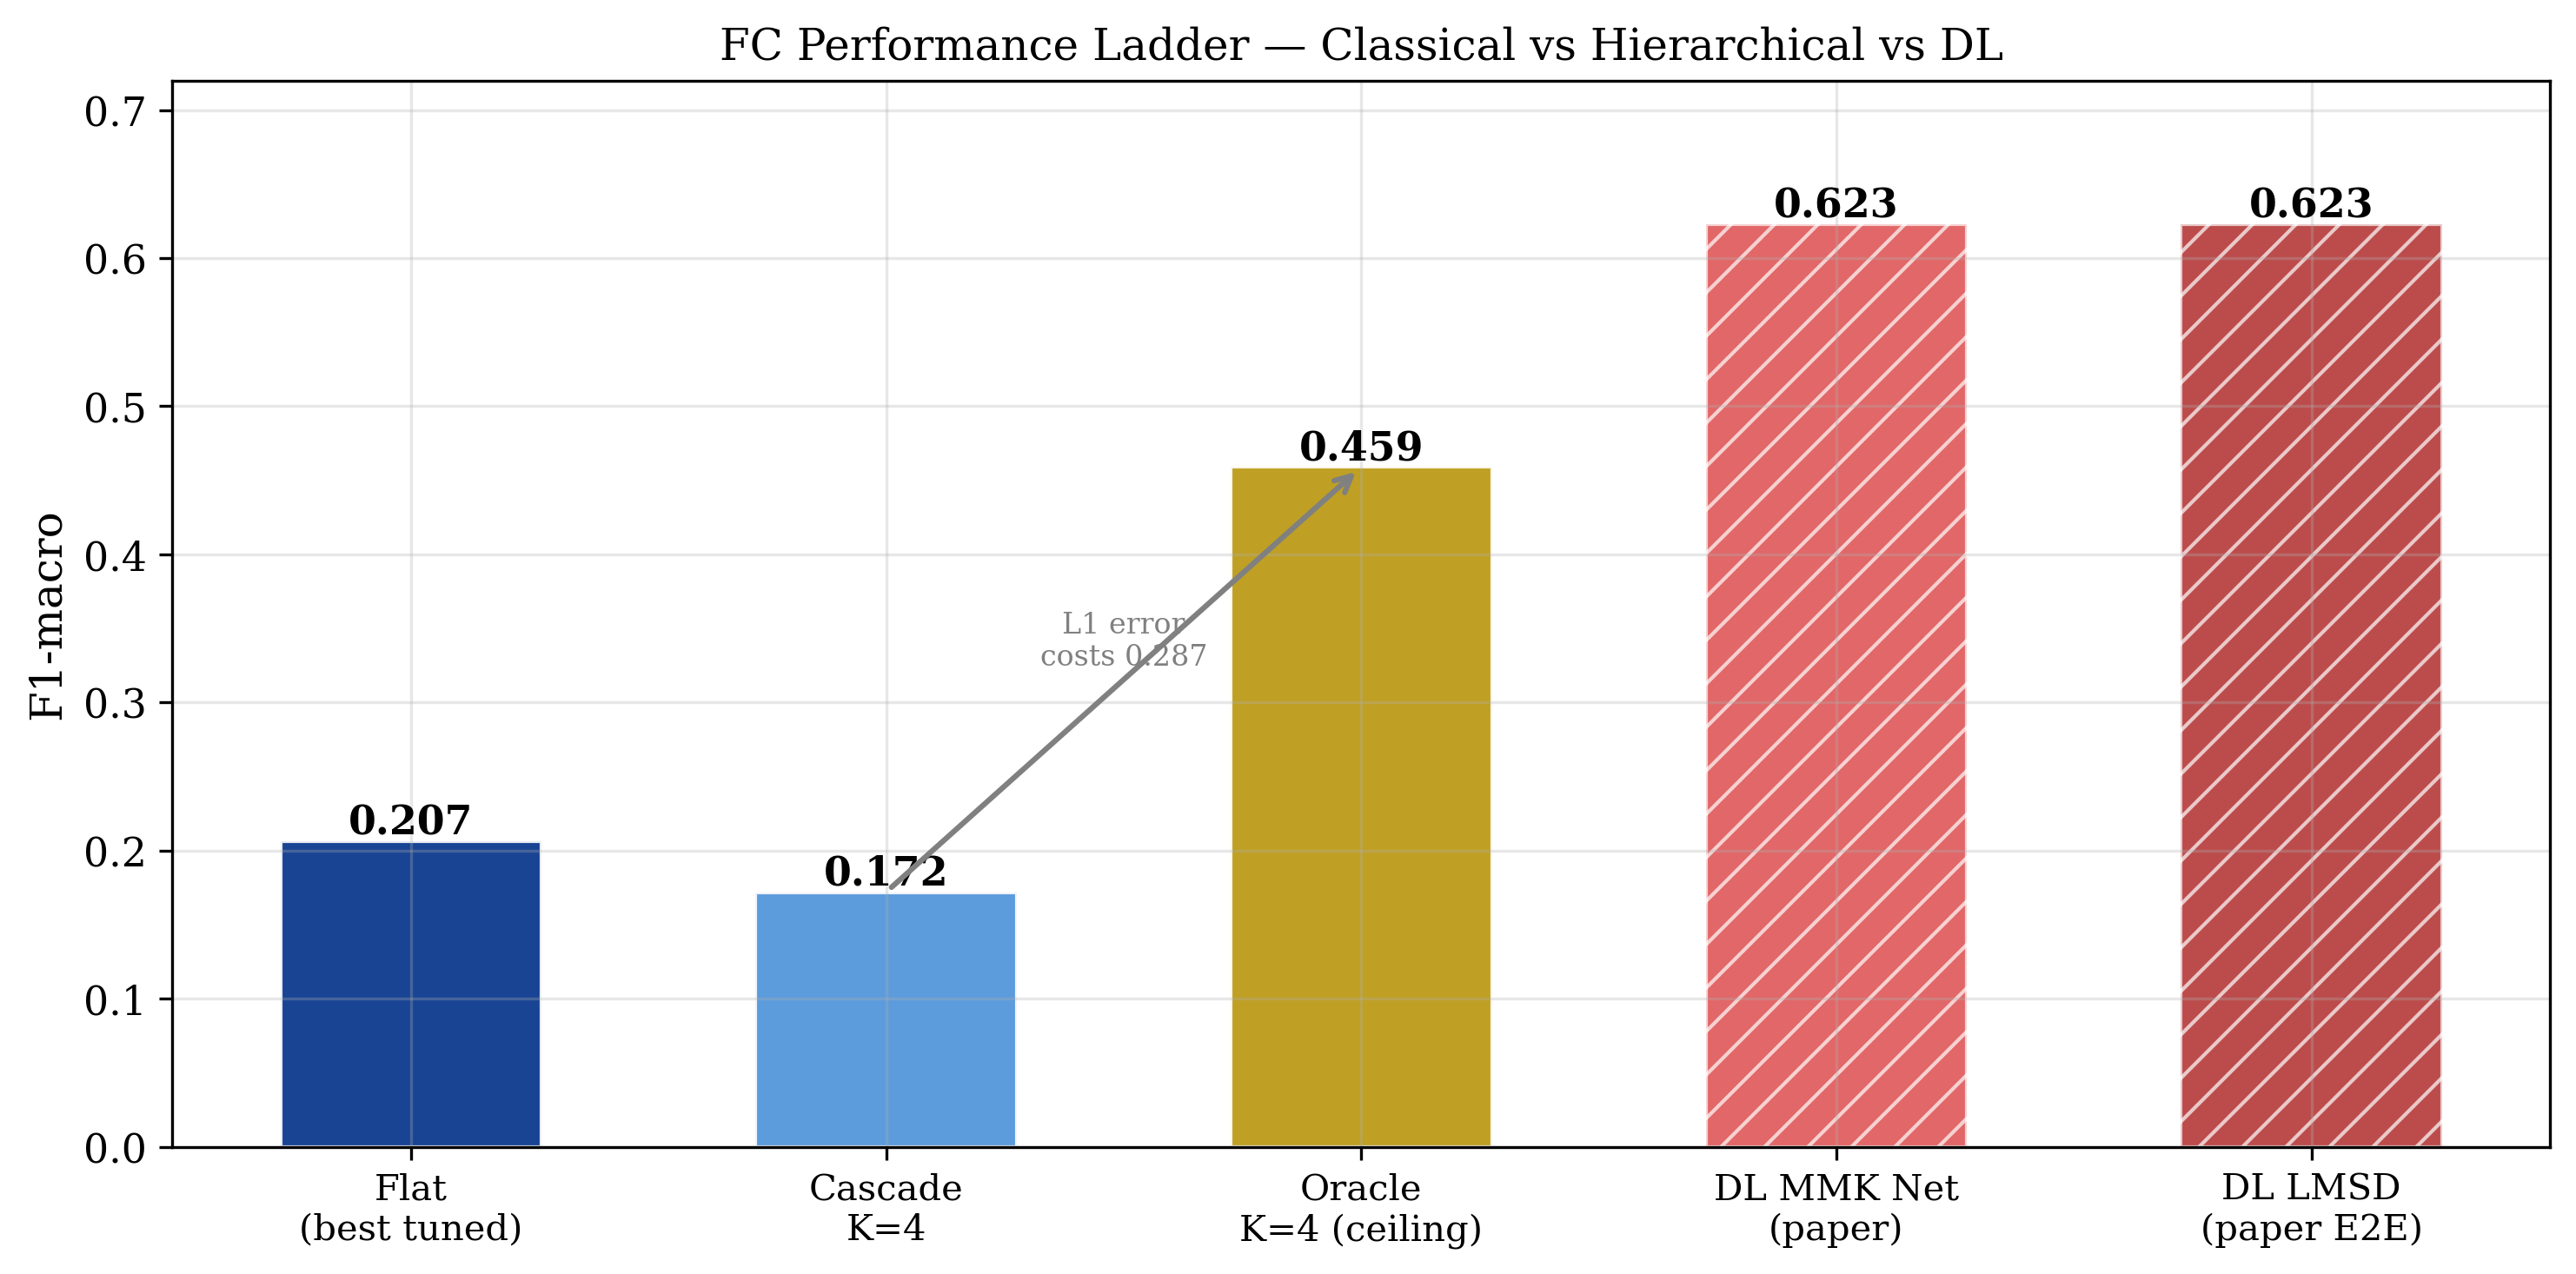
\includegraphics[width=0.95\columnwidth]{fc-oracle-ladder.png}
    \caption{FC performance ladder (notebook~04): flat $\to$ realistic cascade
             $\to$ Oracle ceiling $\to$ indicative DL.}
    \label{fig:fcladder}
\end{figure}

\subsection{End-to-End Diagnosis}
Composing both stages into a 20-class decision (Table~\ref{tab:e2e}), the cascade
AD$\to$FC reaches $F1=0.131$, beating a direct 20-class classifier ($0.113$) and
recovering AD recall of $0.688$. The error decomposition
(Fig.~\ref{fig:e2eerr}) is the key diagnostic: of all cascade predictions, $50\%$
are correct, $15.3\%$ are Stage-1 false negatives (faulty flights labeled
healthy---the safety-critical mode), $14.7\%$ are Stage-1 false positives, and
$20.0\%$ are Stage-2 wrong-type errors. \textbf{Fault typing (S2) is thus the
single largest error source}, confirming that FC---not detection---is where the
pipeline must improve.

\begin{table}[t]
    \centering
    \caption{End-to-end diagnosis (macro-$F1$ over 20 classes, notebook~05).}
    \label{tab:e2e}
    \footnotesize
    \begin{tabular}{llcc}
        \toprule
        \textbf{Architecture} & \textbf{Repr.} & \textbf{F1$_{20}$} & \textbf{AD recall} \\
        \midrule
        Direct 20-class        & $F_{++}$ & 0.113 & 0.509 \\
        \textbf{Cascade AD$\to$FC} & $F_{++}$ & \textbf{0.131} & 0.688 \\
        \midrule
        LMSD (DL, indicative)~\cite{lmsd2025} & raw & 0.623 & 0.837 \\
        \bottomrule
    \end{tabular}
\end{table}

\begin{figure*}[t]
    \centering
    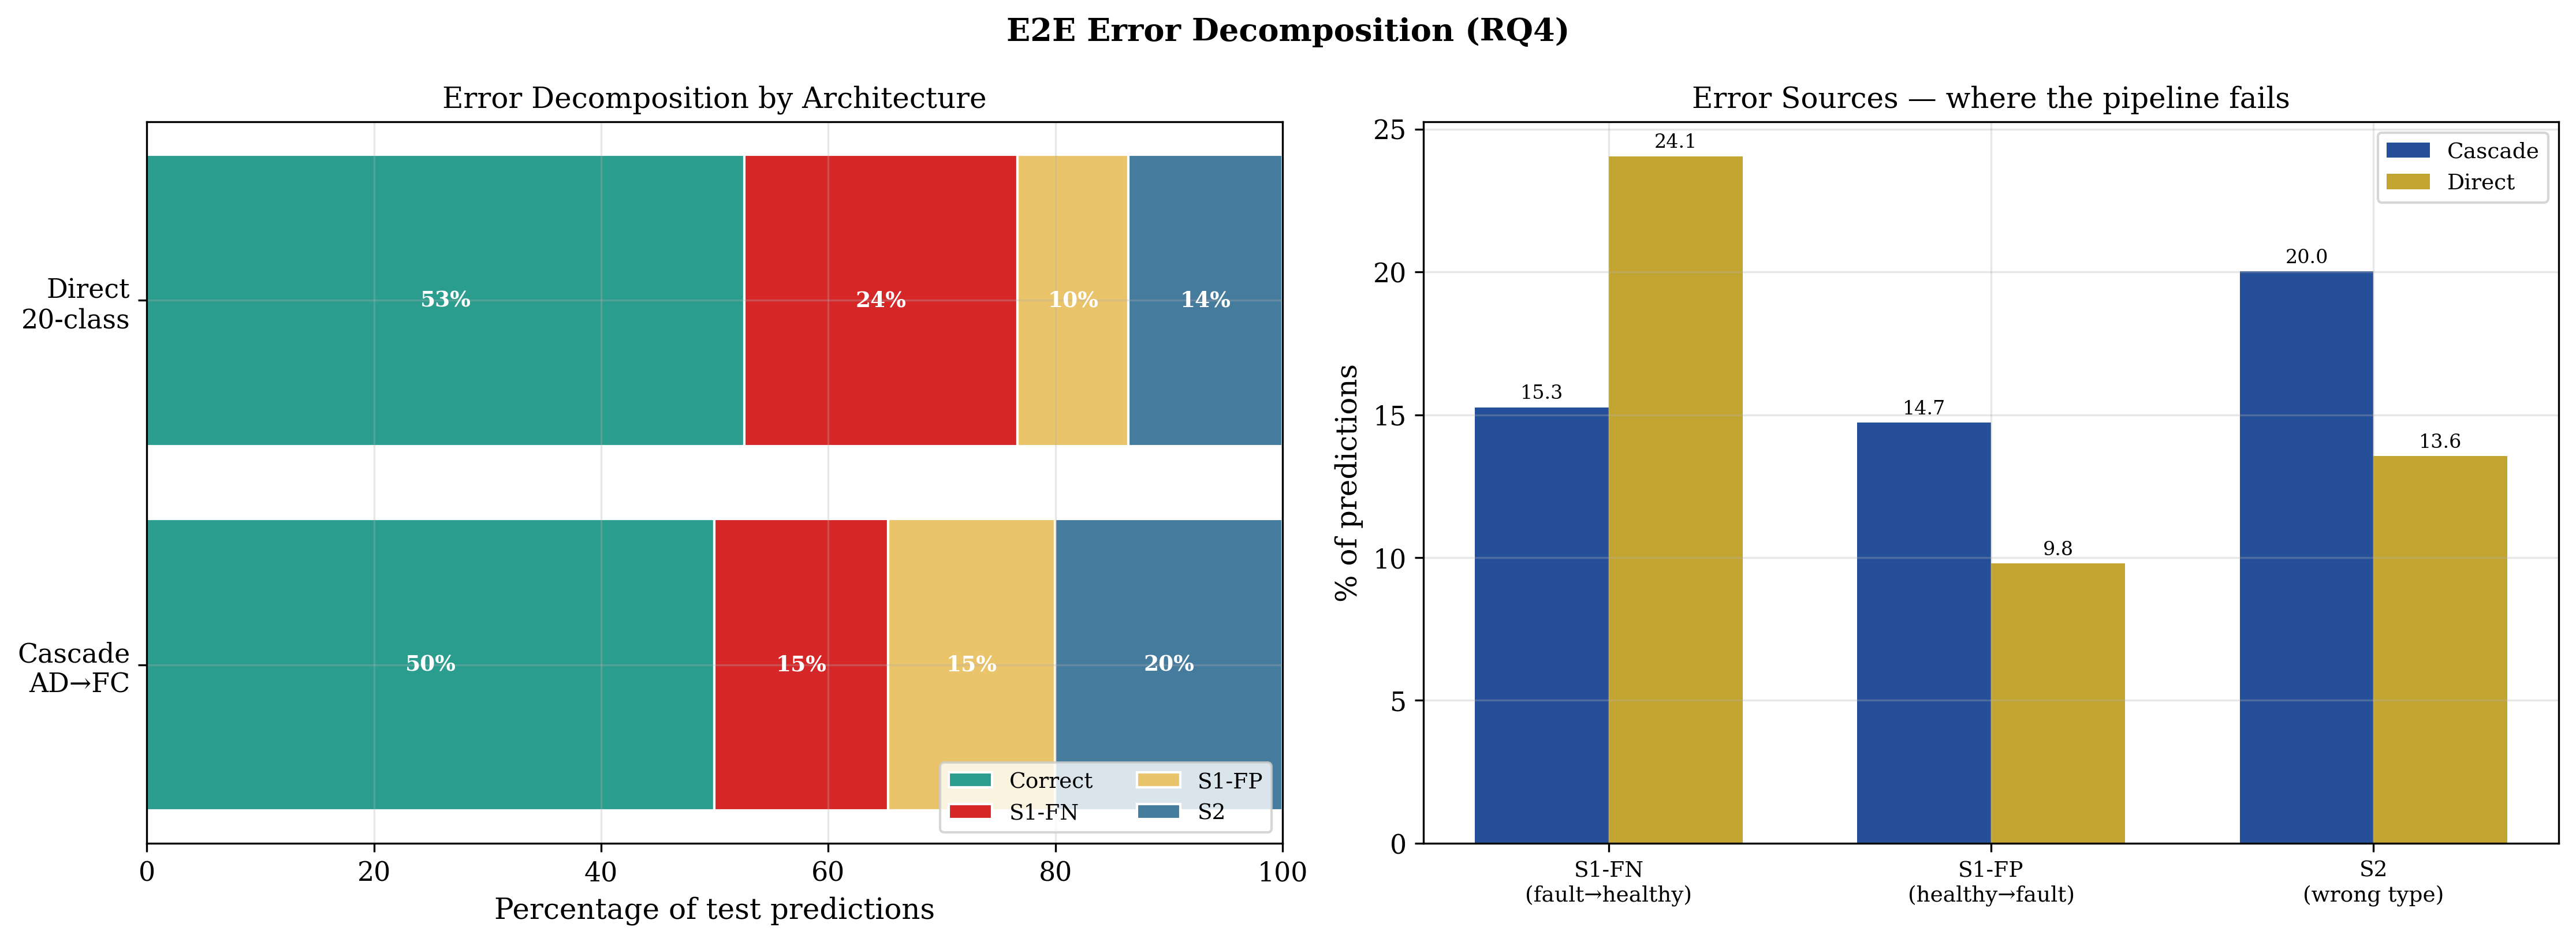
\includegraphics[width=0.9\textwidth]{e2e-error-decomposition.png}
    \caption{E2E error decomposition (notebook~05). Left: error budget by
             architecture. Right: error sources; for the cascade, Stage-2
             wrong-type errors ($20\%$) are the largest, identifying fault
             classification as the bottleneck.}
    \label{fig:e2eerr}
\end{figure*}

% ─────────────────────────────────────────────────────────────────────────────
\section{Discussion}
\label{sec:discussion}
\textbf{Answering the research questions.} For \textbf{RQ1}, the answer is yes: a
tuned classical ensemble on global statistics detects anomalies competitively
($F1=0.703$, within $1.8$ points of MMK~Net), is interpretable, and trains on a
laptop---enough to move part of a fleet toward condition-based inspection. For
\textbf{RQ2}, the answer is largely no: even with feature engineering and an Oracle
hierarchy, FC tops out at $F1=0.459$, leaving most minority faults only partially
recognized. The system is fit for \emph{triage} (sick vs.\ healthy) but not yet
for \emph{prescription} (which part to fix). Both outcomes match our hypothesis:
the difference is explained by target-component sparsity
(Fig.~\ref{fig:sparsity})---global statistics retain the whole-flight health state
needed for AD but discard the low-variance local signatures needed for FC.

\textbf{Relation to prior work.} The qualitative pattern---global context helps
AD, local micro-patterns help FC---is corroborated by the convolutional-
transformer line of NGAFID research~\cite{convtok2023} and by our own ablation, in
which global-attention ConvTokMHSA fails to beat flat XGBoost on FC. The specific
DL gap magnitudes, however, derive from a preprint later withdrawn over
metric-computation flaws~\cite{lmsd2025}; we therefore treat them as provisional.
A retraction at the state of the art arguably makes a transparent, reproducible
classical baseline with honest cross-validated variance more valuable, not less.

\textbf{Tools surveyed.} The project used the open-source Python stack:
NumPy/pandas for munging, scikit-learn~\cite{sklearn2011} for the linear and
distance models, pipelines, and fold-safe preprocessing; XGBoost~\cite{xgboost2016}
as the best flat classical model and gain-based feature selector; and
MiniRocket~\cite{minirocket2021} and tsfresh~\cite{tsfresh2018} for temporal-shape
features. The dedicated time-series transforms inflated the feature space by one
to two orders of magnitude for only marginal FC gain---a strong empirical signal
that fault signatures are local events that generic features dilute, pointing
toward locally restricted deep learning (Keras/TensorFlow) as the principled next
tool, which we surveyed but left to future work.

\textbf{Limitations and future work.} Results use the 19-class benchmark subset;
the full 36-class NGAFID is harder. The Oracle $K{=}4$ figure is an upper bound,
not a deployable number, and the DL reference points inherit the reliability
problem of the withdrawn source. The error decomposition makes the priority
unambiguous: fault typing is the bottleneck. The clearest next steps are (i) a
locally restricted temporal CNN trained on raw sequences to test whether the FC
gap is genuinely temporal; (ii) re-running the benchmark once corrected DL results
are published; and (iii) tackling the $38{:}1$ imbalance directly with resampling
or cost-sensitive losses.

% ─────────────────────────────────────────────────────────────────────────────
\section{Conclusion}
\label{sec:conclusion}
Classical machine learning on global flight statistics delivers a deployable,
interpretable anomaly screen for general-aviation condition-based maintenance
today ($F1=0.703$, within $1.8$ points of a published temporal model), but
reliable fault attribution remains the unsolved half: the classical ceiling is
$F1=0.459$, and the end-to-end bottleneck is fault typing. Because
fault-discriminative information is sparse and low-variance, invisible to global
statistics, the indicated next step is a locally restricted temporal deep model,
evaluated against a re-validated benchmark. All code and notebooks are available
at \texttt{https://github.com/Barbosa12/NGAFID}.

% ─────────────────────────────────────────────────────────────────────────────
\bibliographystyle{IEEEtran}
\bibliography{bib/references}

\end{document}
